\documentclass[11pt,tikz,border=5pt]{standalone}

\usepackage{amsmath}
\usetikzlibrary{arrows.meta, decorations.pathreplacing}


\begin{document}
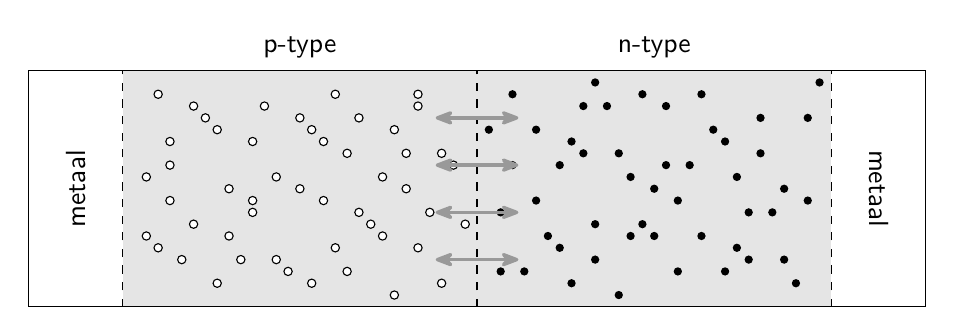
\begin{tikzpicture}[scale=1.5]
  \fill[black!10!white] (0, 0) rectangle (6, 2);

  \foreach \x/\y in {
      1.5/1.0, 2.2/0.6, 0.8/1.5, 1.1/0.8, 2.5/1.7, 1.9/0.3, 0.4/1.2, 0.6/0.7, 2.0/1.6, 2.7/0.2, 1.3/1.1, 1.0/0.4, 2.4/1.3, 1.7/0.9, 0.3/1.8, 0.4/0.9, 1.8/1.8, 2.5/0.5, 1.1/1.4, 1.4/0.3, 2.8/1.2, 2.1/0.7, 0.7/1.6, 0.5/0.4, 1.9/1.3, 2.6/0.8, 1.2/1.7, 0.9/0.6, 2.3/1.5, 1.6/0.2, 0.2/1.1, 0.2/0.6, 1.6/1.5, 2.3/0.1, 0.9/1.0, 1.3/0.4, 2.7/1.3, 2.0/0.8, 0.6/1.7, 0.8/0.2, 2.2/1.1, 2.9/0.7, 1.5/1.6, 1.1/0.9, 2.5/1.8, 1.8/0.5, 0.4/1.4, 0.3/0.5, 1.7/1.4, 2.4/1.0
    } {
      \draw[fill=white] (\x, \y) circle (1pt);
    }
  \foreach \x/\y in {
      1.0/1.9, 1.4/0.7, 2.8/1.6, 2.1/0.3, 0.7/1.2, 0.5/0.9, 1.9/1.8, 2.6/0.4, 1.2/1.3, 0.8/0.2, 2.2/1.1, 1.5/0.6, 0.1/1.5, 0.2/0.8, 1.6/1.7, 2.3/0.4, 0.9/1.3, 1.2/0.1, 2.6/1.0, 1.9/0.6, 0.5/1.5, 0.7/0.5, 2.1/1.4, 2.8/0.9, 1.4/1.8, 1.0/0.7, 2.4/1.6, 1.7/0.3, 0.3/1.2, 0.4/0.3, 1.8/1.2, 2.5/0.8, 1.1/1.7, 1.5/1.0, 2.9/1.9, 2.2/0.5, 0.8/1.4, 0.6/0.6, 2.0/1.5, 2.7/0.2, 1.3/1.1, 1.0/0.4, 2.4/1.3, 1.7/0.9, 0.3/1.8, 0.2/0.3, 1.6/1.2, 2.3/0.8, 0.9/1.7, 1.3/0.6
    } {
      \fill (3 + \x, \y) circle (1pt);
    }

  \draw (-.8, 0) rectangle (6.8, 2);
  \draw[dashed] (3, 0) -- (3, 2);
  \draw[dashed] (0, 0) -- (0, 2);
  \draw[dashed] (6, 0) -- (6, 2);
  \node[rotate=90] at (-.4, 1) {\sffamily metaal};
  \node[rotate=-90] at (6.4, 1) {\sffamily metaal};

  \node[above=1pt] at (1.5, 2) {\sffamily p-type};
  \node[above=1pt] at (4.5, 2) {\sffamily n-type};

  \foreach \y in {.4, .8, 1.2, 1.6} {
  \draw[<->, >={Stealth[round]}, very thick, black!40!white] (2.65, \y) -- (3.35, \y);
  }
\end{tikzpicture}
%
%
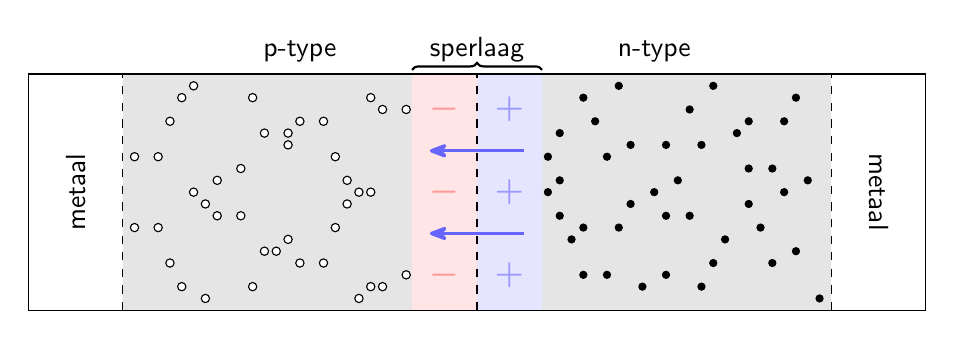
\begin{tikzpicture}[scale=1.5]
  \fill[black!10!white] (0, 0) rectangle (6, 2);

  \begin{scope}
    \fill[red!10!white] (2.45, 0) rectangle (3, 2);
    \foreach \y in {0.3, 1.0, 1.7} {
        \node[red!40!white] at (2.725, \y) {\large$\boldsymbol{-}$};
      }
    \clip (0, 0) rectangle (2.45, 2);
    \foreach \x/\y in {
        2.7/1.5, 2.0/0.1, 0.6/1.0, 0.7/0.9, 2.1/1.8, 2.8/0.5, 1.4/1.4, 1.1/0.2, 2.5/1.1, 1.8/0.7, 0.4/1.6, 0.3/0.7, 1.7/1.6, 2.4/0.3, 1.0/1.2, 1.3/0.5, 2.7/1.4, 2.0/1.0, 0.6/1.9, 0.5/0.2, 1.9/1.1, 2.6/0.6, 1.2/1.5, 0.8/0.8, 2.2/1.7, 1.5/0.4, 0.1/1.3, 0.1/0.7, 1.5/1.6, 2.2/0.2, 0.8/1.1, 1.2/0.5, 2.6/1.4, 1.9/0.9, 0.5/1.8, 0.7/0.1, 2.1/1.0, 2.8/0.6, 1.4/1.5, 1.0/0.8, 2.4/1.7, 1.7/0.4, 0.3/1.3, 0.4/0.4, 1.8/1.3, 2.5/0.9, 1.1/1.8, 1.4/0.6, 2.8/1.5, 2.1/0.2
      } {
        \draw[fill=white] (\x, \y) circle (1pt);
      }
  \end{scope}


  \begin{scope}
    \fill[blue!10!white] (3, 0) rectangle (3.55, 2);
    \foreach \y in {0.3, 1.0, 1.7} {
        \node[blue!40!white] at (3.275, \y) {\large$\boldsymbol{+}$};
      }
    \clip (3.55, 0) rectangle (6, 2);
    \foreach \x/\y in {
        0.7/1.1, 0.6/1.0, 2.0/1.9, 2.7/0.5, 1.3/1.4, 0.9/0.3, 2.3/1.2, 1.6/0.8, 0.2/1.7, 0.3/0.2, 1.7/1.1, 2.4/0.7, 1.0/1.6, 1.3/0.9, 2.7/1.8, 2.0/0.4, 0.6/1.3, 0.8/0.6, 2.2/1.5, 2.9/0.1, 1.5/1.0, 1.1/0.3, 2.5/1.2, 1.8/0.8, 0.4/1.7, 0.4/0.8, 1.8/1.7, 2.5/0.4, 1.1/1.3, 1.4/0.2, 2.8/1.1, 2.1/0.6, 0.7/1.5, 0.5/0.5, 1.9/1.4, 2.6/1.0, 1.2/1.9, 0.9/0.7, 2.3/1.6, 1.6/0.3, 0.2/1.2, 0.2/0.5, 1.6/1.4, 2.3/0.9, 0.9/1.8, 1.2/0.7, 2.6/1.6, 1.9/0.2, 0.5/1.1, 0.7/0.8
      } {
        \fill (3 + \x, \y) circle (1pt);
      }
  \end{scope}

  \draw (-.8, 0) rectangle (6.8, 2);
  \draw[dashed] (3, 0) -- (3, 2);
  \draw[dashed] (0, 0) -- (0, 2);
  \draw[dashed] (6, 0) -- (6, 2);
  \node[rotate=90] at (-.4, 1) {\sffamily metaal};
  \node[rotate=-90] at (6.4, 1) {\sffamily metaal};

  \node[above=1pt] at (1.5, 2) {\sffamily p-type};
  \node[above=1pt] at (4.5, 2) {\sffamily n-type};
  \node[above=1pt] at (3, 2) {\sffamily sperlaag};
  \draw[yshift=1pt,thick, decorate,decoration={brace}] (2.45, 2) -- (3.55, 2);

  \foreach \y in {.65, 1.35} {
  \draw[<-, >={Stealth[round]}, very thick, blue!60!white] (2.6, \y) -- (3.4, \y);
  }
\end{tikzpicture}
\end{document}
